
% Copyright 2020 by Robert Hildebrand
%This work is licensed under a
%Creative Commons Attribution-ShareAlike 4.0 International License (CC BY-SA 4.0)
%See http://creativecommons.org/licenses/by-sa/4.0/

%\documentclass[../open-optimization/open-optimization.tex]{subfiles}
%\begin{document}

\chapter{Pemrograman Matematis}

\begin{outcome}
\begin{itemize}
\item Mengkaji sebuah masalah pengantar
\item Mengidentifikasi alasan untuk mempelajari riset operasi
\item Mendefinisikan ``pemrograman matematis''
\item Mengenal berbagai penerapan alat-alat dalam buku ini
\item Menjelajahi berbagai jenis model optimisasi dan jenis-jenis yang akan dibahas dalam buku ini
\end{itemize}
\end{outcome}
\section{Skenario Pemanasan}
\label{sec:shirt-warmup}

Bayangkan Anda merintis sebuah perusahaan pakaian baru dan memutuskan untuk menjual kaus. Anda telah membuka sebuah toko di Roanoke dan, berdasarkan riset pasar, memperkirakan permintaan untuk akhir pekan mendatang:

\begin{itemize}
    \item \textbf{Jumat}: 5 kaus  
    \item \textbf{Sabtu}: 10 kaus  
    \item \textbf{Minggu}: 7 kaus  
\end{itemize}

Pemasok Anda dapat mengirimkan kaus dalam satu hari; artinya, pesanan yang dibuat pada hari Kamis akan tiba pada hari Jumat, dan demikian seterusnya. Sebagai pemilik usaha, Anda perlu memutuskan berapa banyak kaus yang harus dipesan dan kapan setiap pesanan harus dibuat agar permintaan harian terpenuhi tanpa menyimpan persediaan berlebih. Gambar~\ref{fig:shirt-timeline} menunjukkan waktunya: setiap pesanan tiba satu hari setelah dibuat, sehingga pesanan hari Kamis melayani pelanggan hari Jumat.

\begin{figure}[h]
\centering
\begin{tikzpicture}[
  day/.style={draw=black!60, rounded corners=2pt, fill=blue!6, minimum width=1.9cm, minimum height=0.85cm, font=\small},
  ord/.style={-{Stealth}, thick, draw=orange!80!black},
  lab/.style={font=\scriptsize, text=black!70}]
  \node[day] (thu) at (0,0) {Kam};
  \node[day] (fri) at (2.4,0) {Jum};
  \node[day] (sat) at (4.8,0) {Sab};
  \node[day] (sun) at (7.2,0) {Min};
  \node[lab, below=1pt of fri] {permintaan 5};
  \node[lab, below=1pt of sat] {permintaan 10};
  \node[lab, below=1pt of sun] {permintaan 7};
  \draw[ord] (thu.north) to[bend left=35] node[lab, above] {pesanan tiba esok hari} (fri.north);
  \draw[ord] (fri.north) to[bend left=35] (sat.north);
  \draw[ord] (sat.north) to[bend left=35] (sun.north);
\end{tikzpicture}
\caption{Pesanan yang dibuat pada suatu hari tiba keesokan harinya, sehingga keputusan pemesanan dan permintaan saling berkaitan sepanjang akhir pekan.}
\label{fig:shirt-timeline}
\end{figure}

\textbf{Mendefinisikan Masalah}

Untuk menangani tantangan ini, Anda perlu memikirkan dua faktor utama secara strategis:

\begin{itemize}
    \item \textbf{Jumlah Pesanan}: Berapa banyak kaus yang dipesan setiap hari.
    \item \textbf{Tingkat Persediaan}: Berapa banyak kaus yang tetap tersedia pada akhir setiap hari.
\end{itemize}

Anda dapat mendefinisikan keputusan-keputusan tersebut menggunakan variabel:
\begin{itemize}
    \item Jadikan jumlah kaus yang Anda pesan pada suatu hari sebagai variabel keputusan. Misalnya, Anda dapat melacak jumlah kaus yang dipesan pada hari Kamis, Jumat, dan Sabtu.
    \item Definisikan variabel untuk menyatakan jumlah kaus yang tersedia pada akhir setiap hari.
\end{itemize}

Tujuan Anda adalah memenuhi permintaan yang diproyeksikan sambil mengendalikan biaya. Biaya dapat mencakup:
\begin{itemize}
    \item Biaya pemesanan kaus.
    \item Biaya penyimpanan persediaan.
    \item Penalti karena kehabisan stok.
\end{itemize}

\textbf{Menyempurnakan Skenario}

Seiring pertumbuhan usaha Anda, kerumitan tambahan dapat muncul. Misalnya:
\begin{itemize}
    \item Biaya pemesanan kaus dapat berbeda dari hari ke hari karena penetapan harga oleh pemasok.
    \item Penyimpanan persediaan dapat menimbulkan biaya gudang.
    \item Anggaran dapat membatasi pengeluaran untuk pesanan.
    \item Anda dapat memperluas lini produk dengan menambahkan celana panjang dan kaus kaki, yang masing-masing memiliki permintaan dan biaya tersendiri.
\end{itemize}

Dengan mendefinisikan variabel dan kendala bagi keputusan-keputusan ini secara jelas, Anda dapat menangani masalah secara sistematis dan menyusun strategi yang optimal. Proses bertahap untuk mendefinisikan masalah, memasukkan perincian dunia nyata, dan menyempurnakan solusi ini merupakan aspek mendasar dalam optimisasi.

\subsection*{Siklus Pengembangan Model}

Contoh bertahap ini menggambarkan siklus pemodelan yang berulang:

\begin{enumerate}
    \item \textbf{Masalah Awal}: Menentukan jumlah pesanan untuk memenuhi permintaan.
    \item \textbf{Pemodelan}: Merumuskan model optimisasi berdasarkan informasi yang tersedia.
    \item \textbf{Solusi}: Menyelesaikan model untuk menemukan rencana pemesanan yang optimal.
    \item \textbf{Informasi Baru}: Memasukkan kerumitan dunia nyata tambahan (biaya yang berubah-ubah, biaya persediaan, kendala anggaran, produk tambahan, dan biaya tetap pemesanan).
    \item \textbf{Penyempurnaan}: Memperbarui model agar mencerminkan informasi baru, lalu menyelesaikannya kembali.
\end{enumerate}

\subsection*{Pengembangan Lebih Lanjut}

Ke depan, skenario ini dapat dikembangkan dengan beberapa cara:

\begin{itemize}
    \item \textbf{Memperluas Usaha ke Toko Baru}: Pembukaan toko tambahan menghadirkan permintaan berbasis lokasi, biaya transportasi, serta koordinasi persediaan di beberapa tempat.
    \item \textbf{Merekrut Staf Baru}: Memasukkan biaya tenaga kerja, kendala penjadwalan, dan tingkat produktivitas ke dalam model.
    \item \textbf{Memproduksi Pakaian Sendiri}: Peralihan ke manufaktur mengharuskan kita memodelkan proses produksi, termasuk pembelian bahan baku, kapasitas mesin, dan waktu pengolahan.
    \item \textbf{Permintaan yang Tidak Pasti}: Dalam kenyataan, permintaan mungkin tidak pasti. Model tingkat lanjut dapat memasukkan unsur stokastik atau menggunakan metode probabilistik untuk menangani keacakan.
\end{itemize}

Dalam buku ini, kita akan berfokus pada model deterministik, yakni model yang semua datanya diketahui dan tetap. Landasan yang kuat dalam model-model ini akan mempersiapkan kita untuk menangani masalah yang lebih kompleks dan melibatkan ketidakpastian serta keacakan pada pembelajaran selanjutnya.

\section{Mengapa Mempelajari Riset Operasi?}
\label{sec:why-OR}

Tanpa disadari, Anda sudah berinteraksi dengan optimisasi berkali-kali setiap hari. Rute yang disarankan ponsel, harga tiket pesawat, tersedianya barang yang Anda inginkan di toko, jadwal liga olahraga favorit, dan penentuan pasien ginjal yang dipasangkan dengan donor tertentu: di balik semuanya terdapat model optimisasi seperti yang diajarkan buku ini. Bahkan asisten AI yang ramai diberitakan dilatih melalui optimisasi; pencocokan sebuah model bahasa besar merupakan masalah pemrograman nonlinier dengan miliaran variabel.

Riset Operasi (RO), menurut perumusan organisasi profesi INFORMS, adalah disiplin yang menerapkan metode analitis tingkat lanjut untuk membantu menghasilkan keputusan yang lebih baik. Dalam dunia yang sumber dayanya terbatas dan organisasinya menghadapi tantangan kompleks, RO menyediakan alat dan metodologi untuk memodelkan, menganalisis, dan menyelesaikan masalah alokasi optimal atas sumber daya yang langka. Mempelajari RO membekali seseorang dengan pendekatan sistematis dan kuantitatif terhadap pengambilan keputusan, yang sangat berharga dalam industri seperti logistik, keuangan, layanan kesehatan, dan manufaktur.

Dengan memahami RO, Anda memperoleh kemampuan untuk menyusun model matematis bagi sistem dunia nyata sehingga berbagai skenario dapat disimulasikan dan dioptimalkan. Hal ini meningkatkan efisiensi, mengurangi biaya, dan memperbaiki kinerja. Keterampilan yang dikembangkan melalui pembelajaran RO, seperti berpikir kritis, memecahkan masalah, dan menganalisis data, dapat diterapkan di banyak bidang dan sangat dicari dalam perekonomian berbasis data dewasa ini.

Riset Operasi juga menjembatani teori dan praktik. Disiplin ini mengubah konsep matematis yang abstrak menjadi strategi yang dapat dilaksanakan dan berdampak nyata pada keberhasilan organisasi. Baik untuk mengoptimalkan rantai pasok, menjadwalkan penerbangan, maupun mengelola portofolio, penerapan RO sangatlah luas.

\begin{tcolorbox}[colback=green!4!white, colframe=green!45!black,
  title=\textbf{Seberapa besar nilai optimisasi?}]
Penghematan berikut bukanlah sekadar perkiraan hipotetis. Beberapa contoh yang terdokumentasi adalah:
\begin{itemize}
\item Proyek-proyek finalis INFORMS Franz Edelman Award, penghargaan tertinggi di bidang ini untuk karya terapan, telah mendokumentasikan manfaat kumulatif lebih dari \$419 miliar sejak 1972~\cite{informs2026edelman}.
\item Sistem ORION milik UPS mengoptimalkan rute pengiriman bagi puluhan ribu pengemudi; sistem ini mengurangi jarak tempuh sekitar 100 juta mil per tahun, senilai \$300--400 juta per tahun, serta sekitar 100{,}000 metrik ton CO$_2$~\cite{holland2017ups}.
\item Sistem manajemen pendapatan American Airlines, salah satu keberhasilan awal optimisasi berskala besar, diperkirakan menghasilkan \$1,4 miliar selama tiga tahun pada awal 1990-an~\cite{smith1992yield}.
\item Nederlandse Spoorwegen menyusun ulang jadwal kereta nasionalnya dengan optimisasi, dengan proyeksi laba tahunan tambahan sekitar 40 juta euro, dan meraih Edelman Award 2008 atas pencapaian tersebut~\cite{kroon2009dutch}.
\end{itemize}
Pada inti matematisnya, setiap contoh tersebut menggunakan jenis model yang akan Anda pelajari untuk dibangun dalam buku ini.
\end{tcolorbox}

\section{Apa Itu Pemrograman Matematis?}
\label{sec:what-is-MP}

Pemrograman matematis merupakan bidang inti dalam riset operasi yang berfokus pada perumusan dan penyelesaian masalah optimisasi. Bidang ini mencakup pembuatan model matematis yang merepresentasikan proses pengambilan keputusan suatu sistem, dengan tujuan menemukan hasil terbaik yang mungkin dicapai di bawah kendala yang diberikan. Istilah ``pemrograman'' dalam konteks ini berarti penyusunan rencana atau penjadwalan, bukan pemrograman komputer.

\begin{figure}[htbp]
\centering
\begin{tikzpicture}[
  stage/.style={draw=blue!60!black, rounded corners=3pt, fill=blue!5, text width=3.4cm, align=center, font=\small, inner sep=5pt},
  arr/.style={-{Stealth}, thick, draw=black!70}]
  \node[stage] (p) at (0,0) {\textbf{Masalah keputusan nyata}\\ \scriptsize apa yang dibuat, dikirim, dijadwalkan};
  \node[stage, below=0.45cm of p] (m) {\textbf{Model matematis}\\ $\max\; \c^\top\x$ dengan $A\x \le \b$};
  \node[stage, below=0.45cm of m] (sv) {\textbf{Solver (perangkat pemecah)}};
  \node[stage, below=0.45cm of sv, fill=green!6, draw=green!50!black] (d) {\textbf{Keputusan + jaminan}\\ \scriptsize sebuah rencana dan mutu rencana itu};
  \draw[arr] (p) -- (m);
  \draw[arr] (m) -- (sv);
  \draw[arr] (sv) -- (d);
\end{tikzpicture}
\caption{Alur kerja pemrograman matematis.}
\label{fig:mp-pipeline}
\end{figure}
Inti pemrograman matematis adalah fungsi tujuan: sebuah ekspresi matematis yang mendefinisikan kriteria yang hendak dioptimalkan, misalnya meminimumkan biaya atau memaksimumkan laba. Variabel keputusan merepresentasikan pilihan yang tersedia, sedangkan kendala mencerminkan batasan atau persyaratan masalah, seperti kapasitas sumber daya atau ketentuan peraturan.

Terdapat berbagai jenis pemrograman matematis, yang masing-masing sesuai untuk jenis masalah yang berbeda:

\begin{itemize}
    \item \textbf{Pemrograman Linear (LP)}: Menangani masalah yang fungsi tujuan dan kendalanya sama-sama linier.
    \item \textbf{Pemrograman Bilangan Bulat (IP)}: Melibatkan variabel keputusan yang nilainya harus berupa bilangan bulat.
    \item \textbf{Pemrograman Nonlinier (NLP)}: Menangani masalah dengan fungsi tujuan atau kendala nonlinier.
    \item \textbf{Pemrograman Dinamis (DP)}: Menguraikan masalah menjadi submasalah yang lebih sederhana dan sangat berguna untuk proses pengambilan keputusan bertahap.
\end{itemize}

Pemrograman matematis menyediakan kerangka kerja yang andal untuk mengoptimalkan sistem kompleks dan mengambil keputusan berdasarkan informasi. Kerangka ini memadukan unsur matematika, ekonomi, dan ilmu komputer untuk menghasilkan solusi yang efisien sekaligus efektif.

\section{Penerapan}

Riset operasi dan pemrograman matematis memiliki beragam penerapan di berbagai industri dan sektor:

\begin{itemize}
    \item \textbf{Transportasi dan Logistik}: Mengoptimalkan penentuan rute dan penjadwalan kendaraan pengiriman, mengurangi biaya transportasi, dan meningkatkan efisiensi rantai pasok.
    \item \textbf{Manufaktur}: Merampingkan proses produksi, mengelola tingkat persediaan, dan menjadwalkan mesin guna memaksimumkan produktivitas serta meminimumkan limbah.
    \item \textbf{Keuangan}: Optimisasi portofolio, penilaian risiko, dan penganggaran modal untuk meningkatkan kinerja keuangan dan mengelola ketidakpastian.
    \item \textbf{Layanan Kesehatan}: Mengalokasikan sumber daya seperti staf dan peralatan, menjadwalkan operasi, dan mengelola arus pasien guna meningkatkan mutu layanan serta mengurangi waktu tunggu.
    \item \textbf{Sektor Energi}: Mengoptimalkan pembangkitan dan distribusi listrik, merencanakan integrasi energi terbarukan, dan mengelola konsumsi energi.
    \item \textbf{Telekomunikasi}: Merancang dan mengoptimalkan jaringan, mengalokasikan lebar pita, serta meningkatkan keandalan dan efisiensi sistem komunikasi.
    \item \textbf{Pertanian}: Merencanakan rotasi tanaman, mengoptimalkan penggunaan pupuk dan air, serta mengelola rantai pasok produk pertanian.
    \item \textbf{Sektor Publik}: Perencanaan kota, logistik tanggap darurat, dan analisis kebijakan untuk meningkatkan layanan publik serta pemanfaatan sumber daya.
    \item \textbf{Kecerdasan Buatan}: Melatih model pembelajaran mesin, termasuk model bahasa besar yang mendasari ChatGPT dan Claude, dengan meminimumkan fungsi kerugian menggunakan teknik pemrograman nonlinier.
\end{itemize}

\begin{figure}[h]
\centering
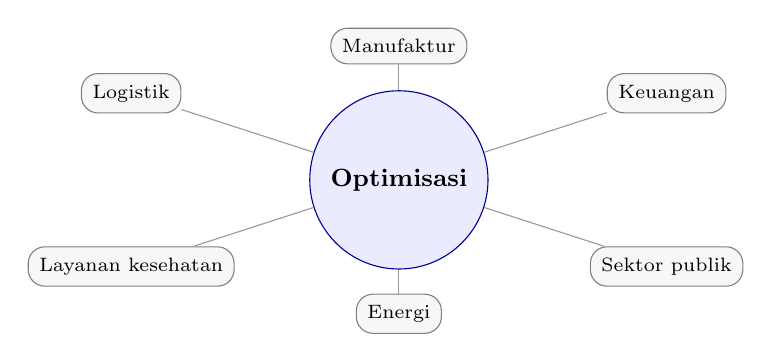
\begin{tikzpicture}[
  hub/.style={draw=blue!60!black, fill=blue!8, circle, font=\small\bfseries, inner sep=6pt},
  sec/.style={draw=black!50, rounded corners=6pt, fill=black!3, font=\scriptsize, inner sep=4pt},
  sp/.style={draw=black!40}]
  \node[hub] (c) at (0,0) {Optimisasi};
  \node[sec] (a) at (-3.4,1.1) {Logistik};
  \node[sec] (b) at (0,1.7) {Manufaktur};
  \node[sec] (f) at (3.4,1.1) {Keuangan};
  \node[sec] (h) at (-3.4,-1.1) {Layanan kesehatan};
  \node[sec] (e) at (0,-1.7) {Energi};
  \node[sec] (g) at (3.4,-1.1) {Sektor publik};
  \foreach \n in {a,b,f,h,e,g} \draw[sp] (c) -- (\n);
\end{tikzpicture}
\caption{Perangkat pemodelan yang sama muncul di berbagai sektor; hanya kata-kata dalam ceritanya yang berubah.}
\label{fig:or-sectors}
\end{figure}

\begin{tcolorbox}[colback=blue!4!white, colframe=blue!55!black,
  title=\textbf{Studi kasus dalam buku ini}]
Di sepanjang buku, kotak studi kasus mengisahkan model optimisasi yang benar-benar
diterapkan; setiap kisah menyertakan model yang dipublikasikan beserta sitasinya:
\begin{itemize}
\item Penempatan hunian berbasis preferensi di koperasi Uruguay (MIP penugasan), \OOCasePage{case:housing-uruguay}.
\item Paket bahan pangan Program Pangan Dunia PBB (LP diet + MILP jaringan), \OOCasePage{case:wfp}.
\item Regionalisasi jaringan pemenuhan pesanan Amazon (MIP desain jaringan), \OOCasePage{case:amazon-regionalization}.
\item Penempatan pesawat tanker pemadam kebakaran hutan di Ontario (IP lokasi cakupan), \OOCasePage{case:wildfire-airtankers}.
\item Pertukaran ginjal dalam program nasional AS dan Britania Raya (IP pemilihan siklus), \OOCasePage{case:kidney-exchange}.
\item Perencanaan muatan truk Walmart (IP pengepakan; Edelman Award 2023), \OOCasePage{case:walmart-loads}.
\end{itemize}
Setiap kotak menyatakan jenis model yang digunakan, asumsi yang dibuat, dan tempat
membaca makalah aslinya.
\end{tcolorbox}

Penerapan-penerapan ini menunjukkan keluwesan dan dampak RO serta pemrograman matematis. Dengan menggunakan alat-alat tersebut, organisasi dapat mengambil keputusan berbasis data yang menghasilkan peningkatan kinerja, penghematan biaya, dan keunggulan bersaing secara berarti. Seiring makin kompleksnya tantangan global, kebutuhan akan tenaga ahli riset operasi terus bertambah.

\Needspace{6\baselineskip}
\section{Jenis-Jenis Masalah Optimisasi}
\label{sec:types-of-optimization}
Kita akan menyatakan kelas-kelas umum utama dari masalah yang dibahas dalam catatan ini. Kelas tersebut ialah Pemrograman Linear (LP), Pemrograman Linear Bilangan Bulat Campuran (MILP), Pemrograman Nonlinier (NLP), dan Pemrograman Nonlinier Bilangan Bulat Campuran (MINLP).  

\begin{center}
\altincludegraphics[width=\linewidth]{Figures/tree-diagram-types}{Diagram pohon yang mengklasifikasikan model optimisasi. Akar 'Model Optimisasi' bercabang menjadi Linier dan Nonlinier; masing-masing kemudian bercabang berdasarkan jenis variabel (kontinu atau bilangan bulat) menjadi empat daun: LP (waktu polinomial), MILP (NP-hard), NLP (bervariasi), dan MINLP (NP-hard).}\par\captionof{figure}{Diagram pohon yang mengklasifikasikan model optimisasi.}\label{fig:tree-diagram-types}% fig-num-auto

\end{center}

Untuk setiap kelas masalah, kita akan menyertakan kelas kompleksitas bagi versi umum masalah tersebut. Kelas kompleksitas dibahas pada bagian selanjutnya dalam buku ini. Meskipun kita akan sering menyatakan bahwa data masukan suatu masalah berasal dari $\R$ (sebagai bilangan real), ketika membahas kompleksitas masalah itu, yang sebenarnya kita maksud ialah bahwa datanya rasional, yakni berasal dari $\Q$ (bilangan rasional yang umumnya dikodekan dalam komputer), dan diberikan dalam pengodean biner.

\begin{warn}
Dalam subbagian berikut, kita akan menggunakan notasi tingkat lanjut yang mungkin belum dikenal pada tahap ini. Notasi matematis tersebut akan dikembangkan di sepanjang buku.

Selain itu, untuk saat ini Anda tidak perlu terlalu mencemaskan definisi khusus dari kelas-kelas kompleksitas. Sementara ini, \polynomial\ dapat dipahami sebagai relatif mudah diselesaikan, sedangkan kelas-kelas lainnya mungkin jauh lebih sulit diselesaikan.
\end{warn}

\Needspace{6\baselineskip}
\section{Pemrograman Linear (LP)}
\label{sec:intro-LP}

Latar belakang, teori, dan contoh pemrograman linear akan diberikan dalam Bagian~I buku ini.
\begin{general}{Pemrograman Linear (LP)}{\polynomial}
\label{general:LP}
Diberikan matriks $A \in \R^{m\times n}$, vektor $\b \in \R^m$, dan vektor $\c \in \R^n$, masalah \emph{pemrograman linear} adalah
\begin{equation}
\label{eq:LP}
\begin{split}
\max \quad & \c^\top \x\\
\st  \quad & A\x \leq \b\\
& \x \geq 0
\end{split}
\end{equation}
\end{general}

Pemrograman linear dapat dinyatakan dalam beberapa bentuk, baik dengan memaksimumkan maupun meminimumkan, serta dengan kendala $\leq, =$ atau $\geq$. Salah satu bentuk yang umum digunakan ialah \emph{bentuk standar}, yang diberikan sebagai
\begin{general}{Bentuk Standar Pemrograman Linear (LP)}{\polynomial}
Diberikan matriks $A \in \R^{m\times n}$, vektor $b \in \R^m$, dan vektor $c \in \R^n$, masalah \emph{pemrograman linear} dalam \emph{bentuk standar} adalah
\begin{equation}
\label{eq:standardLP}
\begin{split}
\max \quad & \c^\top \x\\
\st  \quad & A\x = b\\
& x \geq 0
\end{split}
\end{equation}
\end{general}

\begin{figure}
\includetikz[scale = 0.9]{Figures/LP-figure}
\caption{Kendala dan fungsi tujuan dalam pemrograman linear.}
\end{figure}
%\refincludefigurestatic[Linear programming constraints and objective.][scale = 0.2][h]{wiki/File/linear-programming.png}
% Removed: TikZ version (LP-figure) is used above. Wiki image (CC0, Ylloh 2012) no longer needed.

\section{Pemrograman Linear Bilangan Bulat Campuran (MILP)}
\label{sec:intro-MILP}
Pemrograman linear bilangan bulat campuran akan diperkenalkan dalam \OOIntegerProgrammingReference, sedangkan topik tambahan dibahas dalam Buku~2.
Ingat bahwa notasi $\Z$ berarti himpunan bilangan bulat dan $\R$ berarti himpunan bilangan real. Masalah pertama yang kita kaji di sini ialah \emph{program bilangan bulat biner} (BIP), yang seluruh $n$ variabelnya bersifat biner (bernilai 0 atau 1).

\begin{general}{Pemrograman Bilangan Bulat Biner (BIP)}{\npcomplete}
Diberikan matriks $A \in \R^{m\times n}$, vektor $\b \in \R^m$, dan vektor $\c \in \R^n$, masalah \emph{pemrograman bilangan bulat biner} adalah
\begin{equation}
\label{eq:BIP}
\begin{split}
\max \quad & \c^\top \x\\
\st  \quad & A\x \leq b\\
& \x \in \{0,1\}^n
\end{split}
\end{equation}
\end{general}
Kelas yang sedikit lebih umum ialah kelas \emph{Program Linear Bilangan Bulat} (ILP). Kelas ini sering disebut \emph{Program Bilangan Bulat} (IP), meskipun istilah tersebut dapat membuka kemungkinan adanya bagian nonlinier.

%\refincludefigurestatic[Comparing the LP relaxation to the IP solutions.][scale = 0.3][h]{wiki/File/integer-programming.png}
% Removed: TikZ version (integer-programming) is used below. Wiki image (CC BY-SA 4.0, Fanosta 2019) no longer needed.

\begin{figure}
\includetikz{Figures/integer-programming}
\caption{Perbandingan relaksasi LP dengan solusi IP}
\end{figure}

\begin{general}{Pemrograman Linear Bilangan Bulat (ILP)}{\npcomplete}
Diberikan matriks $A \in \R^{m\times n}$, vektor $\b \in \R^m$, dan vektor $\c \in \R^n$, masalah \emph{pemrograman linear bilangan bulat} adalah
\begin{equation}
\label{eq:ILP}
\begin{split}
\max \quad & \c^\top \x\\
\st  \quad & A\x \leq \b\\
& \x \in \Z^n
\end{split}
\end{equation}
\end{general}

Kelas yang lebih umum lagi ialah \emph{Pemrograman Linear Bilangan Bulat Campuran (MILP)}. Dalam kelas ini terdapat $n$ variabel bilangan bulat $x_1, \dots, x_n \in \Z$ dan $d$ variabel kontinu $x_{n+1}, \dots, x_{n+d} \in \R$. Secara ringkas, kita dapat menuliskannya sebagai $\x \in \Z^n \times \R^d$, dengan $\times$ menyatakan \emph{hasil kali Kartesius} antara dua ruang.   

Di bawah ini, matriks $A$ memiliki $n+d$ kolom, yakni $A \in \R^{m \times (n+d)}$. Perhatikan pula bahwa kita belum memberlakukan syarat nonnegatif pada variabel secara eksplisit. Jika terdapat batasan nonnegatif, batasan itu dapat dianggap sebagai bagian dari deskripsi pertidaksamaan $A\x \leq \b$.
\Needspace{0.33\textheight}
\begin{general}{Pemrograman Linear Bilangan Bulat Campuran (MILP)}{\npcomplete}
Diberikan matriks $A \in \R^{m\times (n+d)}$, vektor $\b \in \R^m$, dan vektor $\c \in \R^{n+d}$, masalah \emph{pemrograman linear bilangan bulat campuran} adalah
\begin{equation}
\label{eq:MILP}
\begin{split}
\max \quad & c^\top x\\
\st  \quad & Ax \leq b\\
& x \in \Z^n \times \R^d
\end{split}
\end{equation}
\end{general}

\Needspace{0.45\textheight}
\section{Pemrograman Nonlinier (NLP)}
\label{sec:intro-NLP}
\begin{general}{NLP}{\nphard}
Diberikan fungsi $f(x)\colon \R^d \to \R$ dan fungsi-fungsi lain $f_i(x)\colon \R^d \to \R$ untuk $i=1, \dots, m$, masalah \emph{pemrograman nonlinier} adalah
\begin{equation}
\label{eq:NLP}
\begin{split}
\min \quad & f(x)\\
\st  \quad & f_i(x) \leq 0  \quad  \text{ untuk } i=1, \dots, m\\
& x \in \R^d
\end{split}
\end{equation}
\end{general}

Pemrograman nonlinier dapat dibedakan menjadi pemrograman konveks dan pemrograman nonkonveks. Keduanya sangat berbeda sehingga penting untuk membedakan satu dari yang lain.
\subsection{Pemrograman Konveks}
Di sini semua fungsinya \textbf{konveks!}
\begin{general}{Pemrograman Konveks}{\polynomial\ \  (biasanya)}
Diberikan fungsi konveks $f(x)\colon \R^d \to \R$ dan fungsi-fungsi konveks $f_i(x)\colon \R^d \to \R$ untuk $i=1, \dots, m$, masalah \emph{pemrograman konveks} adalah
\begin{equation}
\label{eq:convex-programming}
\begin{split}
\min \quad & f(x)\\
\st  \quad & f_i(x) \leq 0  \quad  \text{ untuk } i=1, \dots, m\\
& x \in \R^d
\end{split}
\end{equation}
\end{general}

Perhatikan bahwa pemrograman konveks merupakan perumuman pemrograman linear. Hal ini dapat dilihat dengan menetapkan $f(x) = c^\top x$ dan $f_i(x) = A_i x - b_i$.  

\subsection{Pemrograman Nonlinier Nonkonveks}

Jika fungsi $f$ atau fungsi-fungsi $f_i$ bersifat nonkonveks, masalah ini menjadi masalah pemrograman nonlinier nonkonveks. Terdapat beberapa persoalan kompleksitas yang berkaitan dengannya.

\paragraph{IP sebagai NLP}
Seperti terlihat di atas, kendala kuadratik dapat digunakan untuk membentuk daerah fisibel (himpunan semua solusi yang memenuhi kendala) dengan solusi diskret. Sebagai contoh,
$$
x(1-x) = 0
$$
memiliki tepat dua solusi: $x = 0, x=1$.  
Dengan demikian, kendala kuadratik dapat digunakan untuk memodelkan kendala biner.
\begin{general}{Pemrograman Bilangan Bulat Biner (BIP) sebagai NLP}{\nphard}
Diberikan matriks $A \in \R^{m\times n}$, vektor $b \in \R^m$, dan vektor $c \in \R^n$, masalah \emph{pemrograman bilangan bulat biner} adalah
\begin{equation}
\label{eq:BIP-NLP}
\begin{split}
\max \quad & c^\top x\\
\st  \quad & Ax \leq b\\
& \hcancel[1.5pt]{x \in \{0,1\}^n}\\
& x_i(1-x_i) = 0 \quad \text{ untuk } i=1, \dots, n
\end{split}
\end{equation}
\end{general}

Sebagai alternatif, perhatikan transformasi dengan $x_i \in \{-1,1\}$.
$$
\begin{aligned}
\min & c^\top x \\
\text { dengan syarat } & A x \leq b \\
& x \in \{-1,1\}^n
\end{aligned}
$$
Masalah ini dapat dirumuskan ulang dengan sebuah kendala nonkonveks sebagai
$$
\begin{array}{cl}
\min & c^\top x \\
\text { dengan syarat } & A x \leq b \\
& -1 \leq x_j \leq 1, \quad 1 \leq j \leq n, \\
& \|x\|^2\geq n .
\end{array}
$$

\subsection{Pembelajaran Mesin}

Pada inti matematisnya, pembelajaran mesin adalah proses mempelajari fungsi dari data. Alih-alih meminta seseorang menuliskan aturannya, kita memilih keluarga fungsi $f(x;\theta)$ dengan parameter $\theta$ yang dapat disetel, lalu membiarkan algoritme optimisasi memilih parameter yang paling sesuai dengan data. Fungsi yang dipelajari dapat mengategorikan data (apakah surel ini spam? apakah pemindaian ini menunjukkan tumor?), memprediksi sebuah bilangan (permintaan esok hari atau harga rumah), atau mengelompokkan hal-hal serupa tanpa label (segmen pelanggan atau artikel berita yang berkaitan).

Inilah alasan pembelajaran mesin termasuk dalam buku optimisasi: melatih sebuah model \emph{berarti} menyelesaikan masalah optimisasi, yang biasanya kontinu dan sering kali nonkonveks. Pola yang sama diterapkan di mana-mana:
\begin{itemize}
\item \textbf{Penyaringan spam dan deteksi penipuan}: mengklasifikasikan pesan atau transaksi sebagai sesuatu yang sah atau tidak.
\item \textbf{Peramalan permintaan}: memprediksi penjualan bulan depan dari data historis, cuaca, dan promosi.
\item \textbf{Pengenalan citra}: memberi label pada isi foto, mulai dari membuka kunci ponsel hingga membaca pemindaian medis.
\item \textbf{Rekomendasi}: memprediksi film, lagu, atau produk berikutnya yang akan disukai pengguna.
\item \textbf{Model bahasa besar}: sistem seperti ChatGPT dan Claude dilatih dengan meminimumkan fungsi kerugian atas miliaran parameter, menggunakan teknik pemrograman nonlinier (varian penurunan gradien) yang dijalankan pada skala sangat besar. Matematika untuk melatih teknologi yang paling banyak dibicarakan dalam dasawarsa ini adalah matematika dalam bab-bab pemrograman nonlinier buku ini.
\end{itemize}
Di bawah ini terdapat dua bentuk matematis paling umum dari masalah-masalah tersebut. Keduanya akan kita bahas secara lebih terperinci nanti dalam buku ini.

\subsubsection*{Peminimuman Fungsi Kerugian}

Dalam pembelajaran terawasi, fungsi tujuan ini biasanya berupa fungsi kerugian \( L \) yang mengukur selisih antara prediksi model dan label data yang sebenarnya. Tujuannya ialah menyesuaikan parameter \( \theta \) pada model untuk meminimumkan kerugian tersebut. Secara matematis, hal ini dapat dinyatakan sebagai:
\begin{equation}
\min_{\theta} L(\theta) = \min_{\theta} \frac{1}{N} \sum_{i=1}^{N} l(y_i, f(x_i; \theta))
\end{equation}
dengan \( N \) menyatakan banyaknya titik data, \( l \) merupakan kerugian per titik data (misalnya galat kuadrat untuk regresi atau entropi silang untuk klasifikasi), \( y_i \) adalah label sebenarnya untuk titik data berindeks i, dan \( f(x_i; \theta) \) adalah prediksi model bagi titik data berindeks i dengan parameter \( \theta \).

\begin{figure}[h]
\centering
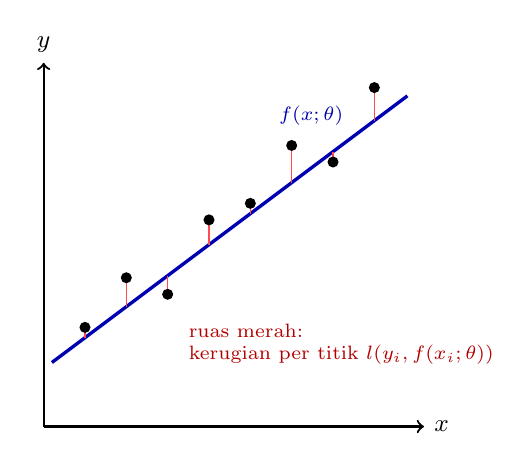
\begin{tikzpicture}[scale=1.05]
  % sumbu
  \draw[->, thick] (0,0) -- (4.6,0) node[right] {\small $x$};
  \draw[->, thick] (0,0) -- (0,4.4) node[above] {\small $y$};
  % garis hasil pencocokan y = 0.75x + 0.7
  \draw[blue!70!black, very thick] (0.1,0.775) -- (4.4,4.0) node[pos=0.85, above left, font=\scriptsize, text=blue!70!black] {$f(x;\theta)$};
  % titik data dan residu
  \foreach \x/\y in {0.5/1.2, 1.0/1.8, 1.5/1.6, 2.0/2.5, 2.5/2.7, 3.0/3.4, 3.5/3.2, 4.0/4.1}{
    \pgfmathsetmacro\fy{0.75*\x + 0.7}
    \draw[red!70, thin] (\x,\y) -- (\x,\fy);
    \fill[black] (\x,\y) circle (1.9pt);
  }
  \node[font=\scriptsize, text=red!70!black, align=left] at (3.6,1.0) {ruas merah:\\ kerugian per titik $l(y_i, f(x_i;\theta))$};
\end{tikzpicture}
\caption{Pembelajaran terawasi sebagai peminimuman kerugian: parameter $\theta$ menggeser dan memiringkan kurva $f(x;\theta)$ hingga ketidakcocokan total dengan data (residu merah) sekecil mungkin.}
\label{fig:ml-loss}
\end{figure}

\subsubsection*{Perumusan Pengelompokan}

Sebaliknya, pengelompokan mempelajari struktur tanpa label sama sekali: data dikelompokkan agar titik-titik dalam kelompok yang sama serupa, sedangkan titik-titik dalam kelompok yang berbeda tidak serupa. Pengecer dapat mengelompokkan pelanggan menjadi beberapa segmen untuk penawaran yang disasar; ahli biologi dapat mengelompokkan gen menurut pola ekspresinya. Salah satu metode yang populer ialah algoritme pengelompokan k-means. Tujuan k-means ialah membagi data menjadi \( k \) klaster dengan meminimumkan jumlah kuadrat dalam klaster (WCSS). Perumusan matematisnya dapat diberikan sebagai:
\begin{equation}
\min_{\mathbf{c}_1, \ldots, \mathbf{c}_k} \sum_{j=1}^{k} \sum_{x_i \in C_j} \left\| x_i - \mathbf{c}_j \right\|^2
\end{equation}
dengan \( C_j \) menyatakan klaster berindeks j dan \( \mathbf{c}_j \) merupakan pusat klaster tersebut.

\begin{figure}[h]
\centering
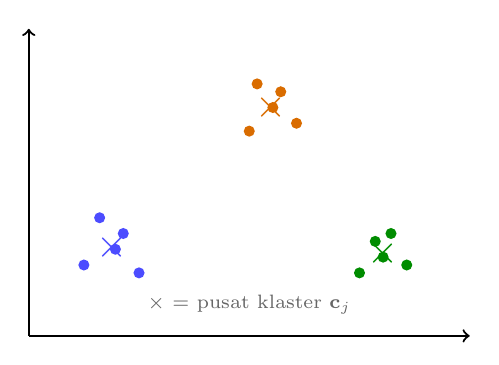
\begin{tikzpicture}[scale=1.0]
  \draw[->, thick] (0,0) -- (5.6,0);
  \draw[->, thick] (0,0) -- (0,3.9);
  % klaster A (biru) di sekitar (1,1)
  \foreach \x/\y in {0.7/0.9, 1.2/1.3, 0.9/1.5, 1.4/0.8, 1.1/1.1}
    \fill[blue!70] (\x,\y) circle (2pt);
  \node[blue!70, font=\Large] at (1.06,1.12) {$\times$};
  % klaster B (jingga) di sekitar (3,2.9)
  \foreach \x/\y in {2.8/2.6, 3.2/3.1, 3.4/2.7, 2.9/3.2, 3.1/2.9}
    \fill[orange!85!black] (\x,\y) circle (2pt);
  \node[orange!85!black, font=\Large] at (3.08,2.9) {$\times$};
  % klaster C (hijau) di sekitar (4.5,1.05)
  \foreach \x/\y in {4.2/0.8, 4.6/1.3, 4.8/0.9, 4.4/1.2, 4.5/1.0}
    \fill[green!55!black] (\x,\y) circle (2pt);
  \node[green!55!black, font=\Large] at (4.5,1.04) {$\times$};
  \node[font=\scriptsize, text=black!60] at (2.8,0.4) {$\times$ = pusat klaster $\mathbf{c}_j$};
\end{tikzpicture}
\caption{Pengelompokan: tanpa label yang diberikan, optimisasi memilih pusat klaster (serta penempatan titik ke pusat tersebut) agar setiap kelompok sepadat mungkin.}
\label{fig:ml-clustering}
\end{figure}

Paparan ringkas ini memberikan gambaran tentang cara masalah pembelajaran mesin dirumuskan secara matematis. Dalam praktiknya, beragam algoritme, kendala, dan regularisasi menambah kerumitan pada perumusan dasar tersebut.

\Needspace{0.45\textheight}
\section{Pemrograman Nonlinier Bilangan Bulat Campuran (MINLP)}
\label{sec:intro-MINLP}

\begin{general}{MINLP}{\nphard}
Pemrograman Nonlinier Bilangan Bulat Campuran (MINLP) memadukan unsur pemrograman bilangan bulat dan pemrograman nonlinier. Dalam MINLP, sebagian atau seluruh variabel keputusan dibatasi agar bernilai bilangan bulat, sedangkan fungsi tujuan atau kendalanya bersifat nonlinier. Masalah MINLP umum dapat dirumuskan sebagai:
\begin{equation}
\label{eq:minlp}
\begin{split}
\min \quad & f(x, y)\\
\st  \quad & g_i(x, y) \leq 0  \quad  \text{ untuk } i=1, \dots, m\\
           & h_j(x, y) = 0    \quad  \text{ untuk } j=1, \dots, p\\
           & x \in \R^n, y \in \Z^k
\end{split}
\end{equation}
dengan $f$ sebagai fungsi tujuan, $g_i$ dan $h_j$ sebagai fungsi kendala, $x$ sebagai vektor variabel kontinu, dan $y$ sebagai vektor variabel bilangan bulat.
\end{general}

MINLP sangat menantang karena adanya nonlinieritas pada fungsi tujuan dan/atau kendala serta sifat diskret sebagian variabel keputusan. MINLP diterapkan di berbagai bidang, seperti optimisasi proses dalam industri, geometri komputasi, dan penyetelan hiperparameter dalam pembelajaran mesin.

\Needspace{0.45\textheight}
\subsection{MINLP Konveks}
Dalam kasus konveks, fungsi tujuan dan kendalanya sama-sama merupakan fungsi konveks. Subkelas ini lebih mudah diselesaikan dibandingkan dengan padanannya yang nonkonveks.
\begin{general}{MINLP Konveks}{\nphard, tetapi \polynomial\ dalam dimensi tetap\  (biasanya)}
Untuk MINLP konveks, masalahnya didefinisikan sebagai:
\begin{equation}
\label{eq:convex-minlp}
\begin{split}
\min \quad & f(x, y) \quad \text{(konveks)}\\
\st  \quad & g_i(x, y) \leq 0  \quad  \text{(kendala konveks)}\\
           & x \in \R^n, y \in \Z^k
\end{split}
\end{equation}
\end{general}
Walaupun tetap menantang, MINLP konveks biasanya lebih mudah ditangani berkat sifat-sifat kekonveksan yang memungkinkan metode penyelesaian lebih efisien.

\subsection{MINLP Nonkonveks}
MINLP nonkonveks jauh lebih sulit karena adanya fungsi nonkonveks, yang dapat menghasilkan banyak minimum lokal.
\begin{general}{MINLP Nonkonveks}{\nphard (bahkan tak dapat diputuskan)}
Masalah MINLP nonkonveks dirumuskan sebagai:
\begin{equation}
\label{eq:nonconvex-minlp}
\begin{split}
\min \quad & f(x, y) \quad
\text{(nonkonveks)}\\
\st \quad & g_i(x, y) \leq 0 \quad \text{(kendala mungkin nonkonveks)}\\
& x \in \R^n, y \in \Z^k
\end{split}
\end{equation}
\end{general}
MINLP nonkonveks menghadirkan tantangan komputasi yang besar karena kemungkinan adanya banyak optimum lokal dan kerumitan bawaan kendala bilangan bulat. Masalah-masalah ini lazim dijumpai dalam penerapan dunia nyata yang keputusannya diskret serta perilaku sistemnya nonlinier dan kompleks.

\subsection*{Kompleksitas dan Penerapan}
Masalah MINLP dikenal memiliki kompleksitas komputasi tinggi, terutama akibat perpaduan nonlinieritas dan keharusan nilai bilangan bulat. Varian nonkonveks, khususnya, bersifat \nphard, sehingga termasuk masalah optimisasi yang paling menantang.

Dalam praktiknya, model MINLP diterapkan secara luas di berbagai bidang. Dalam industri, model ini digunakan untuk proses pengambilan keputusan kompleks seperti optimisasi rantai pasok dan perencanaan produksi. Dalam geometri komputasi, teknik MINLP membantu menyelesaikan masalah seperti pengepakan optimal atau desain tata letak. Dalam pembelajaran mesin, MINLP digunakan untuk tugas seperti pemilihan fitur dan optimisasi hiperparameter yang melibatkan pilihan diskret serta hubungan nonlinier.

Keluwesan model MINLP, bersama dengan kerumitan bawaannya, menjadikannya bidang kajian penting dalam optimisasi.

Daftar lengkap perangkat lunak optimisasi yang disusun menurut jenis masalah (termasuk solver bebas, solver komersial berlisensi akademik, dan antarmuka pemodelan) tersedia dalam \OOSoftwareAppendixReference.

\section{Optimisasi di Bawah Ketidakpastian}

Masalah optimisasi sering melibatkan ketidakpastian pada parameternya, baik akibat galat pengukuran, keragaman data masukan, maupun peristiwa masa depan yang tidak dapat diprediksi. Penanganan ketidakpastian sangat penting untuk mengembangkan solusi yang efektif dalam keadaan dunia nyata. Dua pendekatan utama terhadap optimisasi di bawah ketidakpastian ialah optimisasi stokastik dan optimisasi robust.

\subsection{Optimisasi Stokastik}

Optimisasi stokastik menangani masalah yang sebagian parameternya tidak pasti, tetapi dapat dideskripsikan secara probabilistik. Dalam kerangka ini, proses optimisasi memasukkan nilai harapan, varians, atau karakteristik statistik lain dari parameter yang tidak pasti. Solusi sering dievaluasi berdasarkan kinerjanya terhadap suatu distribusi skenario yang mungkin terjadi. 

Sebagai contoh, dalam manajemen rantai pasok, permintaan yang tidak pasti dapat dimodelkan menggunakan distribusi probabilitas. Sebuah perusahaan dapat berupaya meminimumkan biaya sembari memastikan tingkat layanan yang tinggi dalam berbagai kondisi permintaan. Demikian pula, optimisasi portofolio dalam bidang keuangan sering memperhitungkan imbal hasil masa depan yang tidak pasti dengan memaksimumkan imbal hasil harapan sambil mengelola risiko.

\Needspace{6\baselineskip}
\subsection{Optimisasi Robust}

Sebaliknya, optimisasi robust berfokus pada pembuatan solusi yang berkinerja baik untuk realisasi ketidakpastian dalam kasus terburuk. Alih-alih mengasumsikan distribusi probabilitas tertentu, optimisasi robust menggunakan himpunan ketidakpastian, yang mendefinisikan rentang nilai yang mungkin diambil oleh parameter tidak pasti. Tujuannya ialah menemukan solusi yang fisibel dan efektif bagi semua skenario yang mungkin dalam himpunan ketidakpastian tersebut.

Penerapan optimisasi robust mencakup operasi jaringan listrik, yang mengharuskan pengelolaan ketidakpastian pada permintaan dan pembangkitan energi terbarukan, serta masalah penjadwalan, seperti penjadwalan awak maskapai, yang mengharuskan gangguan diminimumkan dalam berbagai kondisi operasi.

\subsection{Penerapan}

Optimisasi di bawah ketidakpastian memiliki beragam penerapan di berbagai industri:
\begin{itemize}
    \item \textbf{Layanan Kesehatan:} Merancang strategi vaksinasi untuk meminimumkan penyebaran penyakit sembari memperhitungkan tingkat infeksi dan perilaku pasien yang tidak pasti.
    \item \textbf{Transportasi:} Mengelola arus lalu lintas atau jadwal angkutan umum ketika permintaan dan waktu perjalanan tidak pasti.
    \item \textbf{Energi:} Merencanakan investasi dan operasi energi terbarukan ketika kondisi cuaca dan harga energi tidak pasti.
    \item \textbf{Manufaktur:} Memastikan jadwal produksi tahan terhadap gangguan rantai pasok dan keragaman mutu bahan baku.
\end{itemize}

Penanganan kerumitan data yang tidak pasti biasanya membuat masalah-masalah ini jauh lebih sulit daripada padanan deterministiknya. Meskipun metode-metode tersebut andal dan dapat diterapkan pada beragam skenario dunia nyata, buku ajar ini tidak akan berfokus pada optimisasi di bawah ketidakpastian.

\section{Latihan}

\exgroup{Pemanasan}

\begin{ex}{Klasifikasikan: Rencana Produksi}{}
\stars{1} Sebuah perusahaan jus memutuskan berapa liter jus apel $x_1$ dan jus jeruk $x_2$ yang akan diproduksi. Setiap liter jus apel menghasilkan \$2 dan setiap liter jus jeruk menghasilkan \$3. Kapasitas pemerasan memberikan $x_1 + 2x_2 \leq 800$, kapasitas pembotolan memberikan $x_1 + x_2 \leq 600$, dan kedua jumlah tersebut tidak negatif. Perusahaan memaksimumkan pendapatan. Klasifikasikan model ini sebagai LP, ILP/BIP, MILP, NLP, atau MINLP. Tunjukkan dua ciri model (jenis fungsi dan jenis variabel) yang membenarkan jawaban Anda.
\exrefs{\S\ref{sec:intro-LP}, Masalah~\eqref{eq:LP}}
\end{ex}

\begin{ex}{Klasifikasikan: Memilih Proyek}{}
\label{ex:classify-projects}
\stars{1} Sebuah kota dapat mendanai sembarang subhimpunan dari lima proyek taman. Proyek $i$ berbiaya $a_i$ dolar dan memberi manfaat kepada $c_i$ warga, sedangkan anggarannya adalah $b$ dolar. Tetapkan $x_i = 1$ jika proyek $i$ didanai dan $x_i = 0$ jika tidak, lalu perhatikan
\[
\max \Big\{ \sum_{i=1}^5 c_i x_i \;:\; \sum_{i=1}^5 a_i x_i \leq b, \; x_i \in \{0,1\} \Big\}.
\]
Klasifikasikan model ini sebagai LP, ILP/BIP, MILP, NLP, atau MINLP, dan berikan alasannya. Bagaimana klasifikasinya berubah jika kota juga dapat mendanai sebagian dari sebuah proyek?
\exrefs{\S\ref{sec:intro-MILP}, Masalah~\eqref{eq:BIP}}
\end{ex}

\begin{ex}{Klasifikasikan: Mencocokkan Garis}{}
\stars{1} Diberikan titik-titik data $(t_1,y_1), \dots, (t_N,y_N)$, kita memilih kemiringan $m$ dan intersep $q$ untuk meminimumkan
\[
\sum_{i=1}^N (y_i - (mt_i + q))^2 ,
\]
dengan $m, q \in \R$ tanpa batasan. Klasifikasikan model ini sebagai LP, ILP/BIP, MILP, NLP, atau MINLP, dan berikan alasannya. Apakah fungsi tujuan linier terhadap variabel keputusan $m$ dan $q$?
\exrefs{\S\ref{sec:intro-NLP}, Masalah~\eqref{eq:NLP}, \S\ref{sec:intro-LP}}
\end{ex}

\begin{ex}{Klasifikasikan: Gudang dengan Kemacetan}{}
\stars{1} Sebuah perusahaan ritel memutuskan gudang mana dari $k$ calon gudang yang akan dibuka ($y_j \in \{0,1\}$) serta berapa banyak produk $x_j \geq 0$ yang akan dialirkan melalui setiap gudang yang dibuka. Biaya penanganan di gudang $j$ meningkat secara kuadratik terhadap volume, sehingga fungsi tujuan memuat suku $x_j^2$, dan produk hanya dapat mengalir melalui gudang $j$ jika $y_j = 1$. Klasifikasikan model ini sebagai LP, ILP/BIP, MILP, NLP, atau MINLP, dan benarkan jawaban Anda dengan menyebutkan unsur yang menyingkirkan setiap kelas yang lebih sederhana.
\exrefs{\S\ref{sec:intro-MINLP}, Masalah~\eqref{eq:minlp}}
\end{ex}

\exgroup{Masalah inti}

\begin{ex}{Toko Kaus: Variabel dan Satu Kendala}{}
\label{ex:shirt-friday-balance}
\stars{2} Kembali ke toko kaus dalam Bagian~\ref{sec:shirt-warmup}: permintaannya adalah 5 kaus pada hari Jumat, 10 pada hari Sabtu, dan 7 pada hari Minggu; pesanan tiba satu hari setelah dibuat; dan toko memulai hari Kamis tanpa persediaan kaus.
\begin{enumerate}
\item Definisikan variabel keputusan untuk kaus yang dipesan pada hari Kamis, Jumat, dan Sabtu, serta untuk persediaan yang disimpan pada akhir hari Jumat dan Sabtu.
\item Dengan menggunakan variabel Anda, tuliskan satu persamaan linier yang menghubungkan pesanan hari Kamis, permintaan hari Jumat, dan persediaan akhir hari Jumat.
\item Kendala mana dalam model Anda yang mencegah toko kehabisan kaus pada hari Jumat?
\end{enumerate}
\exrefs{\S\ref{sec:shirt-warmup}, Gambar~\ref{fig:shirt-timeline}}
\end{ex}

\begin{ex}{Temukan Unsur-unsurnya: Truk Makanan}{}
\stars{2} Pemilik sebuah truk makanan harus memutuskan berapa banyak taco dan burrito yang akan disiapkan esok hari. Setiap taco menggunakan 0.1 kg daging dan setiap burrito menggunakan 0.25 kg, sedangkan daging yang tersedia hanya 30 kg. Tenaga kerja untuk persiapan dibatasi 10 jam. Taco menghasilkan laba \$2 dan burrito \$3.50. Tanpa menuliskan model lengkap, identifikasikan dengan kata-kata: variabel keputusan, fungsi tujuan, dan setiap kendala. Nyatakan satuan setiap besaran yang Anda sebutkan.
\exrefs{\S\ref{sec:what-is-MP}, Gambar~\ref{fig:mp-pipeline}}
\end{ex}

\begin{ex}{Temukan Unsur-unsurnya: Pusat Bimbingan Belajar}{}
\stars{2} Sebuah pusat bimbingan belajar menyusun jadwal tutor untuk pekan depan. Pusat tersebut dapat mempekerjakan masing-masing dari 12 tutor untuk sejumlah sesi berdurasi satu jam yang harus berupa bilangan bulat, paling banyak 8 sesi per tutor. Pusat itu perlu menyediakan sedikitnya 40 sesi secara keseluruhan dan memiliki anggaran mingguan \$900; tutor $i$ mengenakan biaya $p_i$ dolar per sesi. Pusat tersebut ingin memaksimumkan jumlah sesi dalam batas anggaran. Identifikasikan variabel keputusan, fungsi tujuan, dan kendalanya dengan kata-kata. Kemudian jelaskan kelas model dari Bagian~\ref{sec:types-of-optimization} yang sesuai dengan masalah ini dan mengapa masalah tersebut bukan sekadar LP.
\exrefs{\S\ref{sec:what-is-MP}, \S\ref{sec:types-of-optimization}}
\end{ex}

\exgroup{Konsep dan keterkaitan}

\begin{ex}{Setengah Bus}{}
\stars{2} Model sebuah distrik sekolah menyatakan bahwa armada optimal berjumlah 12.5 bus. Model sebuah toko kaus menyatakan bahwa pesanan optimal berjumlah 2361.4 kaus.
\begin{enumerate}
\item Dalam kasus manakah pembulatan jawaban LP ke bilangan bulat terdekat kemungkinan dapat diterima, dan mengapa?
\item Jelaskan arti persoalan keterbagian bagi pemilihan antara kelas masalah LP dan MILP, serta harga yang harus kita bayar (dalam kesulitan komputasi) ketika mengharuskan variabel bernilai bilangan bulat.
\end{enumerate}
\exrefs{\S\ref{sec:types-of-optimization}, \S\ref{sec:intro-MILP}}
\end{ex}

\begin{ex}{Mengapa Disebut ``Pemrograman''?}{}
\label{ex:programming-term}
\stars{2} Kata ``pemrograman'' dalam pemrograman matematis muncul sebelum perangkat lunak modern. Jelaskan dalam satu atau dua kalimat makna istilah tersebut dalam bidang ini, dan mengapa ``pemrograman linear'' bukan berarti menulis kode komputer secara linier.
\exrefs{\S\ref{sec:what-is-MP}}
\end{ex}

\begin{ex}{Membaca Kisah Keberhasilan}{}
\stars{2} Pilih salah satu keberhasilan terdokumentasi dalam kotak ``Seberapa besar nilai optimisasi?'' di Bagian~\ref{sec:why-OR} (UPS ORION, manajemen pendapatan American Airlines, atau jadwal Nederlandse Spoorwegen). Untuk sistem yang Anda pilih, uraikan: (a) variabel keputusan yang mungkin digunakan, (b) fungsi tujuan yang mungkin dioptimalkan, dan (c) satu kendala yang harus dipatuhi model. Jawaban Anda tidak perlu tepat sepenuhnya; tujuannya ialah menerjemahkan klaim bergaya berita menjadi komponen model.
\exrefs{\S\ref{sec:why-OR}, \S\ref{sec:what-is-MP}}
\end{ex}

\exgroup{Masalah tantangan}

\begin{ex}{Toko Kaus: Model Lengkap}{}
\label{ex:shirt-full-lp}
\stars{3} Rumuskan masalah lengkap pemesanan kaus dari Bagian~\ref{sec:shirt-warmup} sebagai program linear. Permintaan adalah 5 kaus pada hari Jumat, 10 pada hari Sabtu, dan 7 pada hari Minggu. Pesanan yang dibuat pada hari Kamis, Jumat, dan Sabtu tiba keesokan harinya dan masing-masing berbiaya \$8, \$9, dan \$10 per kaus. Setiap kaus yang masih berada di toko pada akhir hari Jumat atau Sabtu menimbulkan biaya penyimpanan \$0.50 untuk malam itu. Toko memulai usaha tanpa persediaan, seluruh permintaan harus dipenuhi tepat waktu, dan sisa kaus setelah hari Minggu diperbolehkan tetapi tidak menghasilkan pendapatan.
\begin{enumerate}
\item Tuliskan LP: variabel keputusan, fungsi tujuan, persamaan keseimbangan persediaan untuk hari Jumat, Sabtu, dan Minggu, serta syarat nonnegatif.
\item Selesaikan model tersebut (dengan perangkat lunak atau penalaran mengenai biaya), lalu laporkan rencana pemesanan optimal dan biaya totalnya.
\item Sebenarnya, variabel-variabel tersebut seharusnya bernilai bilangan bulat. Apakah hal itu berpengaruh di sini? Jelaskan.
\end{enumerate}
\exrefs{\S\ref{sec:shirt-warmup}, \S\ref{sec:intro-LP}, Gambar~\ref{fig:shirt-timeline}}
\end{ex}

\subsubsection*{Solusi Terpilih}

\begin{solution}(Latihan~\ref{ex:classify-projects})
Model ini merupakan program bilangan bulat biner (BIP): fungsi tujuan dan kendala anggarannya linier, sedangkan setiap variabel dibatasi pada $\{0,1\}$. Jika sebagian proyek boleh didanai, gantilah $x_i \in \{0,1\}$ dengan $0 \leq x_i \leq 1$; semua kendala kemudian bersifat linier atas variabel kontinu dan model tersebut menjadi LP.
\end{solution}

\begin{solution}(Latihan~\ref{ex:shirt-friday-balance})
Misalkan $x_T, x_F, x_S$ adalah jumlah kaus yang dipesan pada hari Kamis, Jumat, dan Sabtu, sedangkan $s_F, s_S$ adalah persediaan pada akhir hari Jumat dan Sabtu. Pesanan hari Kamis merupakan seluruh persediaan yang dimiliki toko pada hari Jumat, sehingga keseimbangan hari Jumat adalah
\[
x_T = 5 + s_F .
\]
Kendala $s_F \geq 0$ (bersama persamaan keseimbangan ini) mencegah kehabisan stok pada hari Jumat: kendala tersebut memaksa $x_T \geq 5$.
\end{solution}

\begin{solution}(Latihan~\ref{ex:programming-term})
Di sini, ``pemrograman'' berarti penyusunan rencana atau penjadwalan: sebuah ``program'' merupakan rencana kegiatan, seperti dalam program logistik militer atau susunan acara konser. Pemrograman linear adalah penyusunan rencana optimal dengan menggunakan hubungan linier, dan istilah tersebut diciptakan sebelum pemrograman komputer digunakan secara luas.
\end{solution}

\begin{solution}(Latihan~\ref{ex:shirt-full-lp})
Misalkan $x_T, x_F, x_S \geq 0$ adalah pesanan yang dibuat pada hari Kamis, Jumat, dan Sabtu, sedangkan $s_F, s_S, s_{Sun} \geq 0$ adalah persediaan pada akhir hari. LP-nya adalah
\begin{align*}
\min \quad & 8x_T + 9x_F + 10x_S + 0.5s_F + 0.5s_S\\
\st \quad & x_T = 5 + s_F && \text{(Jumat)}\\
& s_F + x_F = 10 + s_S && \text{(Sabtu)}\\
& s_S + x_S = 7 + s_{Sun} && \text{(Minggu)}\\
& x_T, x_F, x_S, s_F, s_S, s_{Sun} \geq 0.
\end{align*}
Memenuhi permintaan satu kaus pada hari Sabtu dengan memesan pada hari Kamis berbiaya $8 + 0.5 = 8.50$, lebih murah daripada pesanan hari Jumat seharga \$9; memenuhi permintaan satu kaus pada hari Minggu dengan memesan pada hari Kamis berbiaya $8 + 0.5 + 0.5 = 9$, lebih murah daripada \$9.50 (memesan hari Jumat dan menyimpan satu malam) serta \$10 (memesan hari Sabtu). Jadi, rencana optimal memesan semuanya pada hari Kamis: $x_T = 22$, $x_F = x_S = 0$, dengan $s_F = 17$, $s_S = 7$, $s_{Sun} = 0$ dan biaya total $22 \cdot 8 + 0.5(17 + 7) = \$188$. Keharusan nilai bilangan bulat tidak menjadi persoalan dalam kasus ini: permintaannya berupa bilangan bulat dan solusi LP optimal sudah bernilai bilangan bulat, sehingga model LP dan model bilangan bulat memberikan hasil yang sama.
\end{solution}

%
%
%\end{document}
